% !TEX root = ../main.tex
\section{Introduction}
The availability of large scale datasets with detailed annotation, such as
ImageNet~\citep{imagenet}, played a significant role in the recent success of deep learning. The
need for such a large dataset is however a limitation, since its collection requires intensive human
labor. This is also strikingly different from human learning, where new concepts can be learned from
very few examples. One line of work that attempts to bridge this gap is few-shot
learning~\citep{koch2015siamese,matching,proto}, where a model learns to output a classifier given
only a few labeled examples of the unseen classes. While this is a promising line of work, its
practical usability is a concern, because few-shot models only focus on learning novel classes,
ignoring the fact that many common classes are readily available in large datasets.

An approach that aims to enjoy the best of both worlds, the ability to learn from large datasets for
common classes with the flexibility of few-shot learning for others, is {\it \ourproblemsmall}~\citep{lwof}. This combines incremental learning where we want to add new classes without
catastrophic forgetting~\citep{mccloskey1989catastrophic}, with few-shot learning when the new
classes, unlike the base classes, only have a small amount of examples. One use case to illustrate
the problem is a visual aid system. Most objects of interest are common to all users, e.g., cars,
pedestrian signals; however, users would also like to augment the system with additional
personalized items or important landmarks in their area. Such a system needs to be able to learn new
classes from few examples, without harming the performance on the original classes and typically
without access to the dataset used to train the original classes.

In this work we present a novel method for incremental few-shot learning where during meta-learning
we optimize a regularizer that reduces catastrophic forgetting from the incremental few-shot
learning. Our proposed regularizer is inspired by attractor networks~\citep{localist} and can be
thought of as a memory of the base classes, adapted to the new classes. We also show how this
regularizer can be optimized, using recurrent back-propagation~\citep{rbp,rbp2,rbp3} to
back-propagate through the few-shot optimization stage. Finally, we show empirically that our
proposed method can produce state-of-the-art results in incremental few-shot learning on {\it
mini}-ImageNet~\citep{matching} and {\it tiered}-ImageNet~\citep{fewshotssl} tasks.
% !TEX root = ../main.tex
\begin{figure}[t]
\centering
\iflatexml
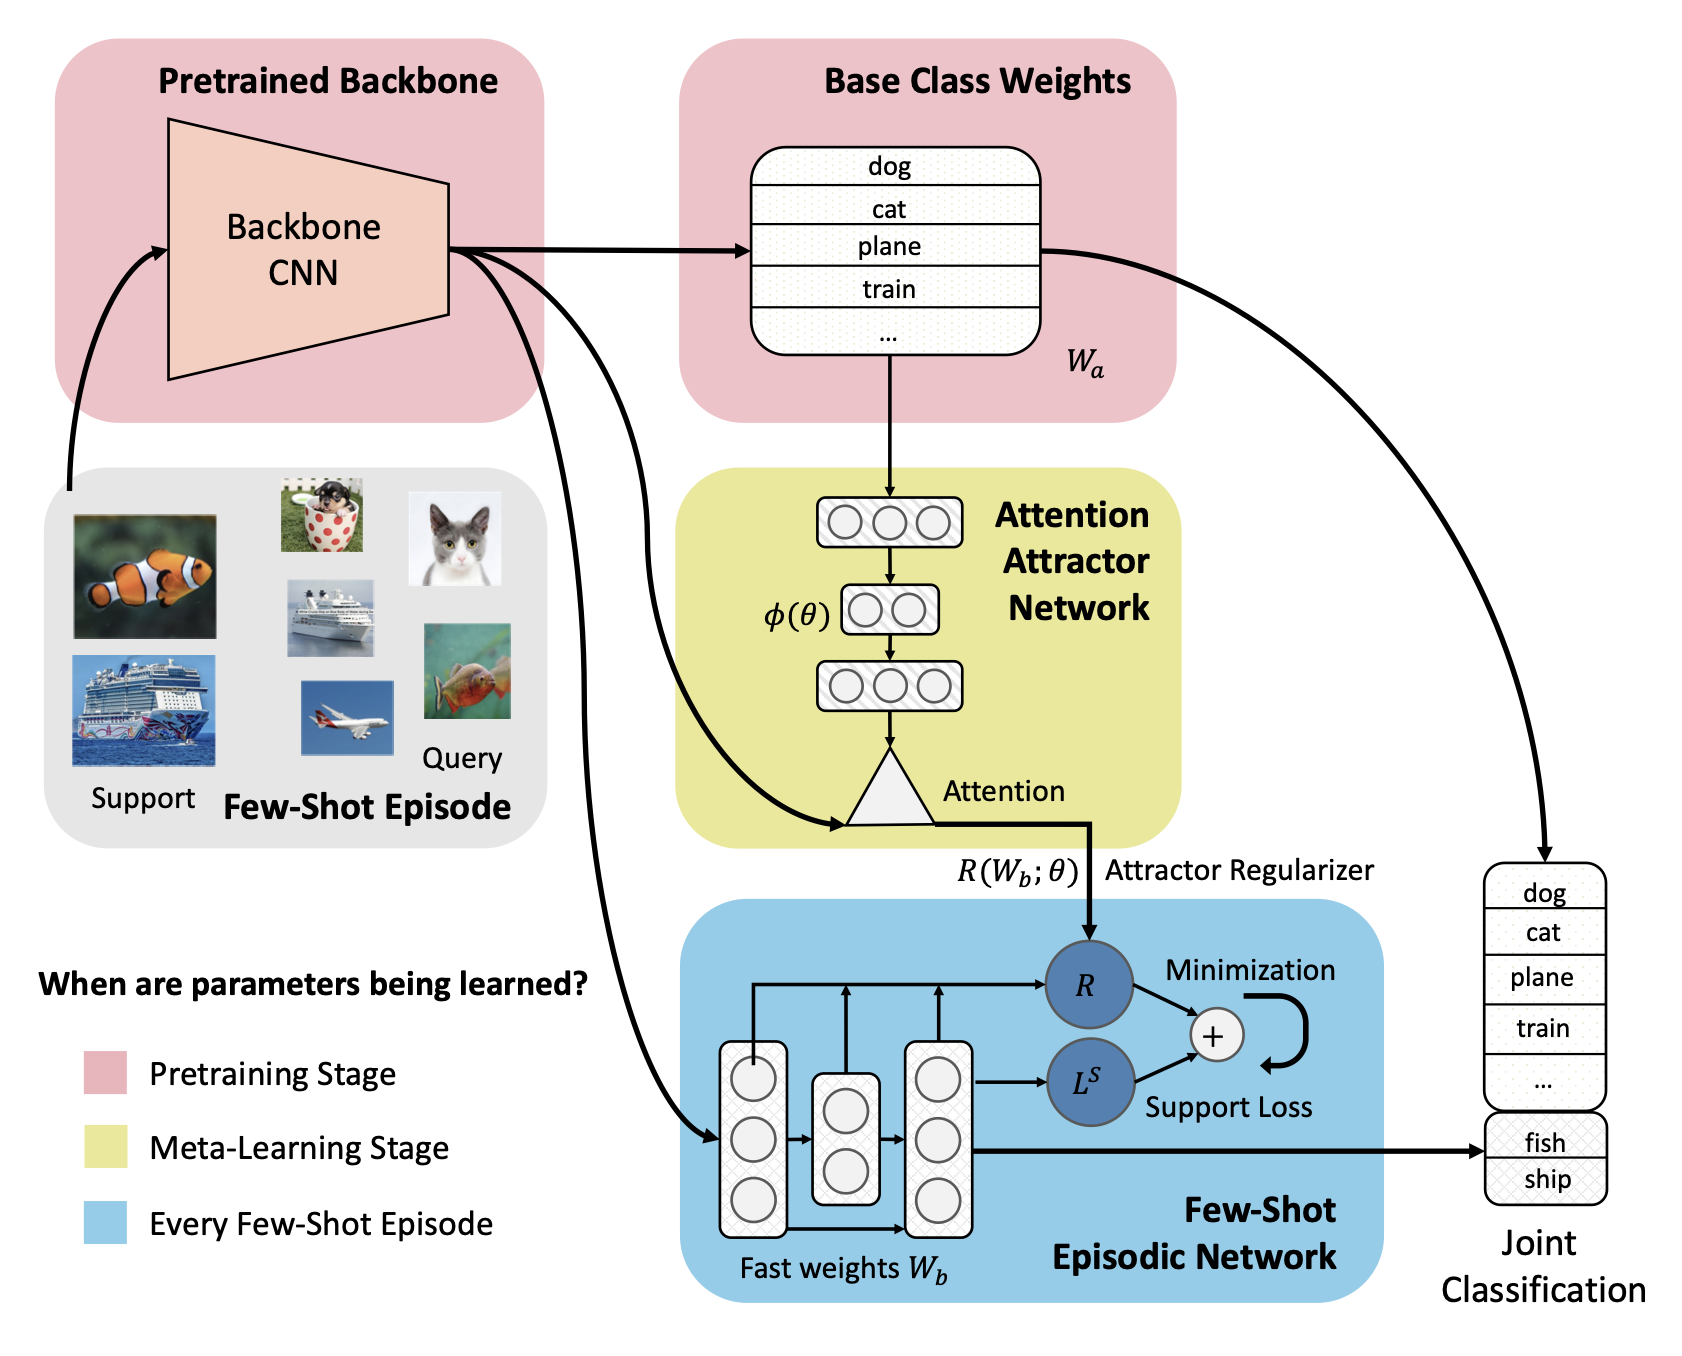
\includegraphics[width=6\textwidth]{figures/mainfig.png}
\else
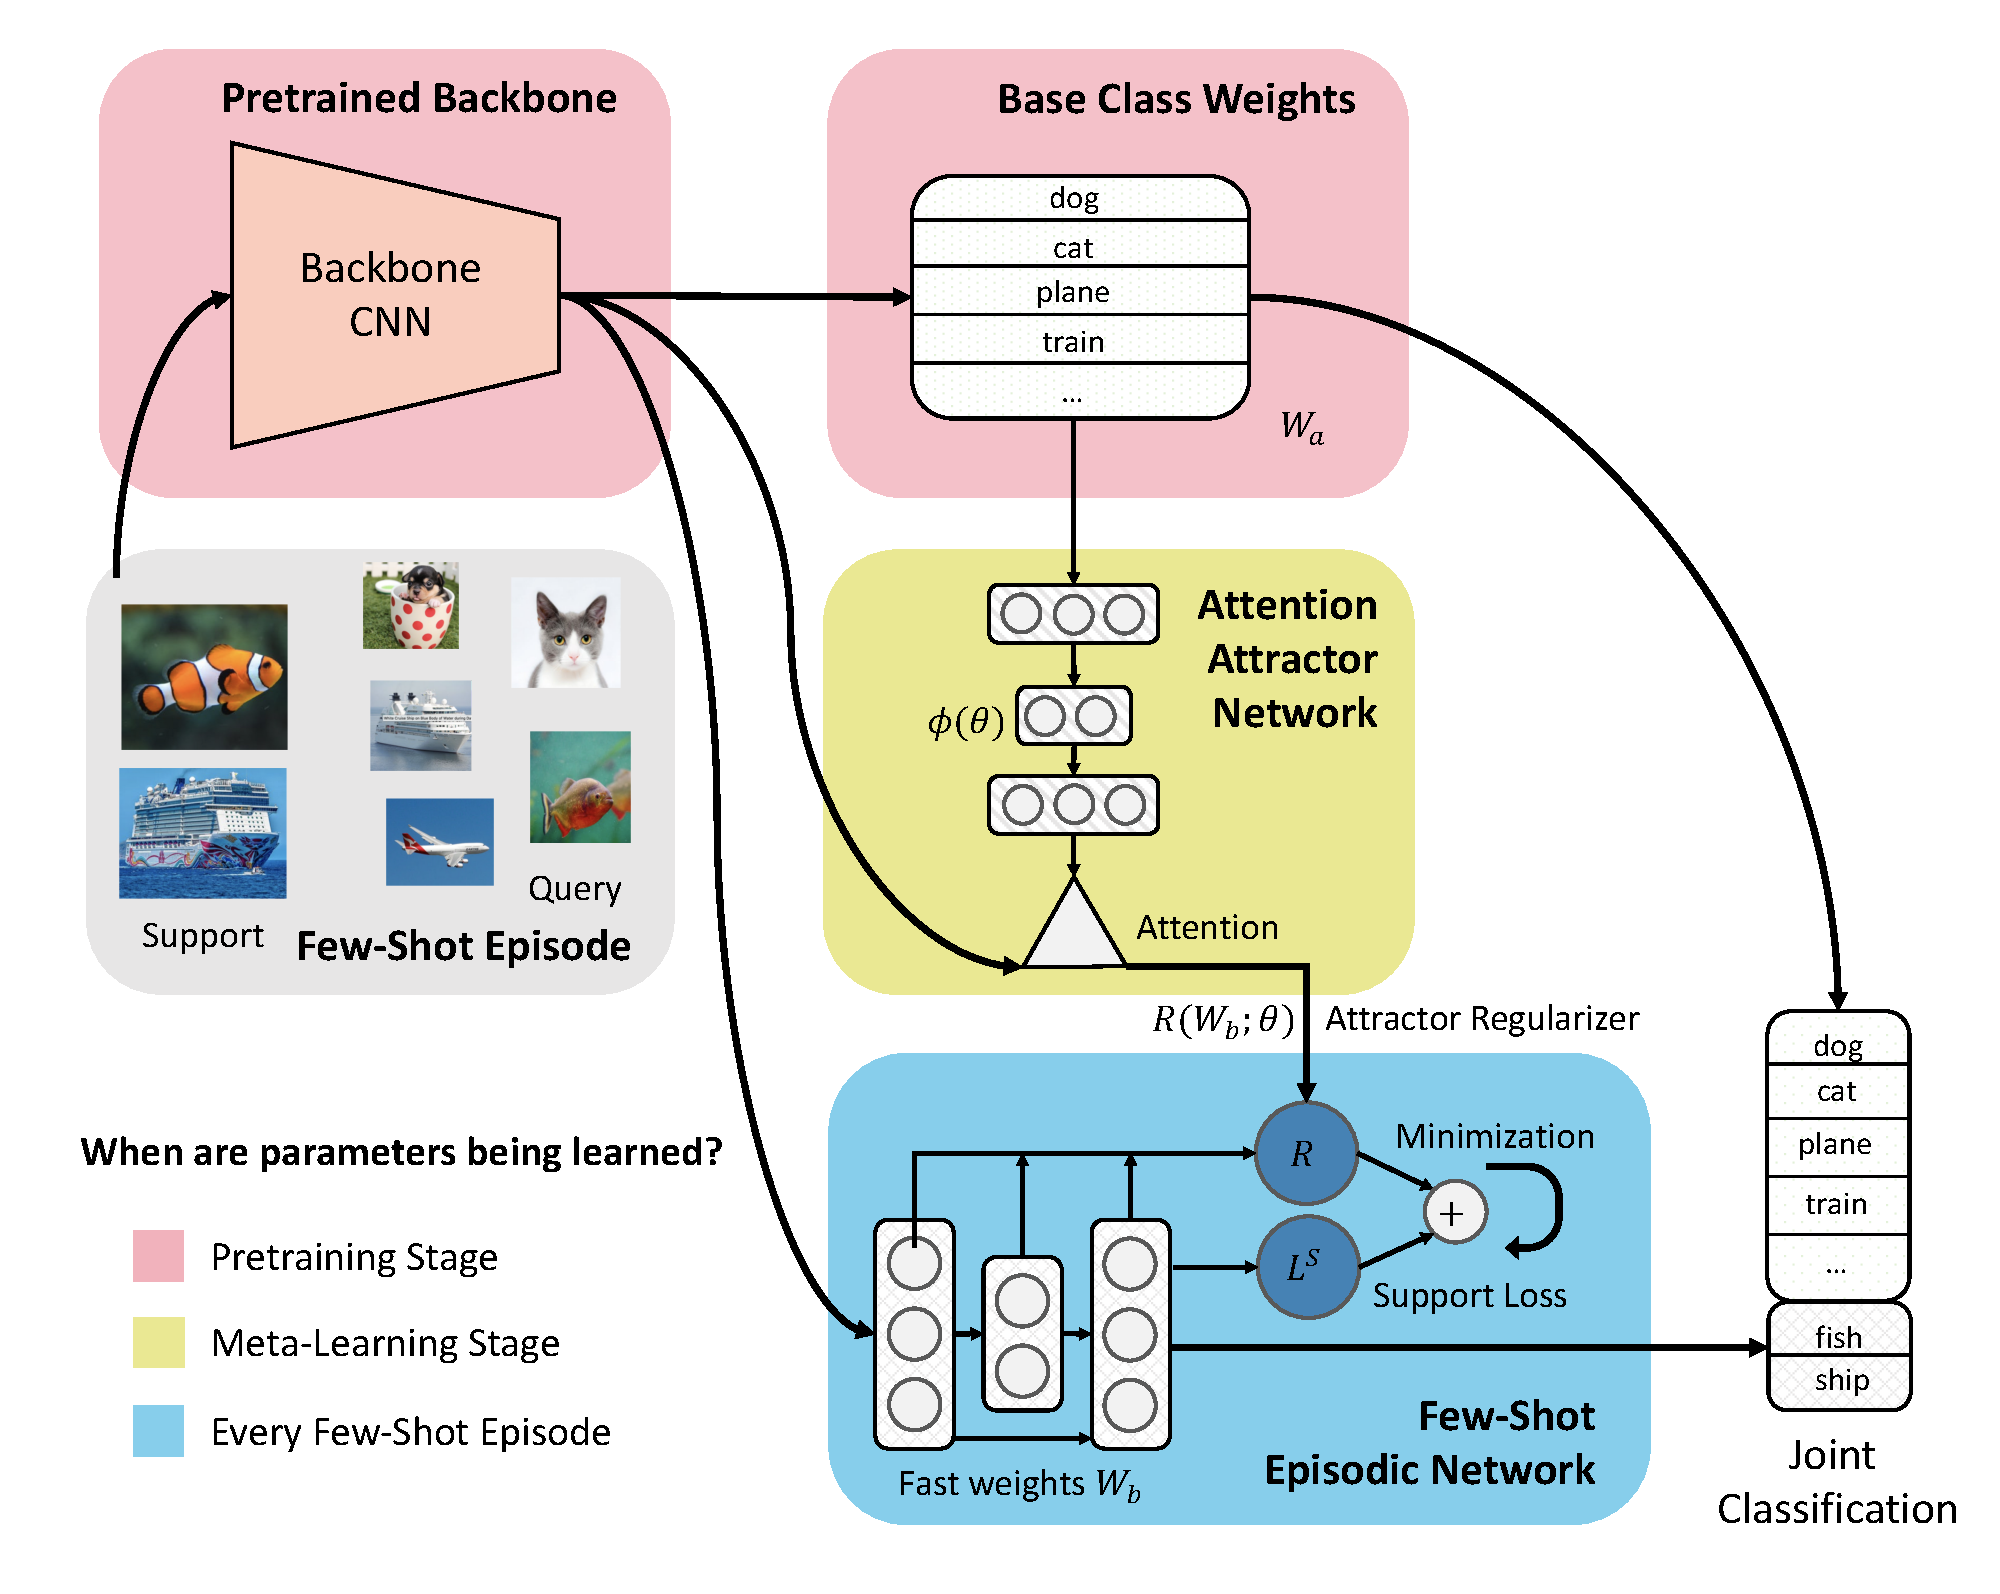
\includegraphics[width=0.7\textwidth,trim={1cm 0 0 0.7cm},clip]{figures/attractor_v4.pdf}
\fi
\caption{Our proposed attention attractor network for incremental few-shot learning.
During pretraining we learn the base class weights $W_a$ and the feature extractor CNN backbone. In
the meta-learning stage, a few-shot episode is presented. The support set only contains novel
classes, whereas the query set contains both base and novel classes. We learn an episodic classifier
network through an iterative solver, to minimize cross entropy plus an additional regularization
term predicted by the attention attractor network by attending to the base classes. The attention
attractor network is meta-learned to minimize the expected query loss. During testing an episodic
classifier is learned in the same way.}
\label{fig:model}
\end{figure}